\documentclass[11pt, a4paper, twoside]{article} %draft

\usepackage{url}
\usepackage{amsmath}
\usepackage{graphicx}
\usepackage{array}
\usepackage{babel,csquotes,xpatch}
\usepackage[backend=bibtex8]{biblatex}
\usepackage{nameref}
\usepackage{xcolor}
\usepackage{tikz}
\usetikzlibrary{arrows,automata}
\usepackage{dirtree}
\usepackage{listings}
\usepackage{packages/listings-golang}
\usepackage{enumitem}

\lstset{
	frame=tb,
	tabsize=4,
	numbers=left,
	numberstyle=\tiny\color{gray},
	basicstyle=\footnotesize
}

%define Javascript language
\lstdefinelanguage{JavaScript}{
	keywords={typeof, new, true, false, catch, function, return, null, catch, switch, var, if, in, while, do, else, case, break},
	keywordstyle=\color{blue}\bfseries,
	ndkeywords={class, export, boolean, throw, implements, import, this, require},
	ndkeywordstyle=\color{darkgray}\bfseries,
	identifierstyle=\color{black},
	sensitive=false,
	comment=[l]{//},
	morecomment=[s]{/*}{*/},
	commentstyle=\color{purple}\ttfamily,
	stringstyle=\color{red}\ttfamily,
	morestring=[b]',
	morestring=[b]"
}



%main colors of CP-MAC app
\definecolor{accent-light}{RGB}{192, 204, 217}
\definecolor{accent-dark}{RGB}{129, 144, 164}

% used to create a square of 0.3cm x 0.3cm to show solor palettes
\newcommand\crule[1][black]{\textcolor{#1}{\rule{0.3cm}{0.3cm}}}


\addbibresource{resources/bibliography.bib}



\begin{document}
% Example of title page for the projects carried out within DEDIS
% Copied from lasec 

% Simply include it in your mastex tex file: 
%        % Example of title page for the projects carried out within DEDIS
% Copied from lasec 

% Simply include it in your mastex tex file: 
%        % Example of title page for the projects carried out within DEDIS
% Copied from lasec 

% Simply include it in your mastex tex file: 
%        \input{cover}


% Updated October 2016


\newcommand{\logoepfl}[0]{
  \begin{center}
    
\includegraphics[width=4cm]{logo_epfl_coul.eps}
  \end{center}
  \vspace{0.3cm}
  \hrule
}
\newcommand{\project}[1]{
  \begin{center}
    \large{#1}
  \end{center}
  \vspace{1cm}
}
\newcommand{\department}[1]{
  \begin{center}
    \large{#1}
  \end{center}
}
\newcommand{\lab}[1]{
  \begin{center}
    \large{#1}
  \end{center}
}
\newcommand{\supervisor}[3]{
  \begin{center}
    \begin{normalsize}{
        \bf #1}\\#2\\#3
    \end{normalsize}
  \end{center}
}
\renewcommand{\author}[1]{
  \begin{center}
    \Large{#1}
  \end{center}
  \vspace{0.5cm}
}
\renewcommand{\title}[1]{
  \vspace{3cm}
  \begin{center}
    \huge{#1}
  \end{center}
  \vspace{1.7cm}
}
\renewcommand{\date}[2]{
  \begin{center}
    \normalsize{#1 #2}
  \end{center}
  \vspace{0.5cm}
}


\thispagestyle{empty}


% begin title page
  \logoepfl
  
  \title{Explore cross-platform mobile platforms}
  
  \author{Louis-Maxence Garret}
  \department{School of Computer and Communication Sciences}
  \lab{Decentralized and Distributed Systems lab}
  \project{Master Optional Project}
  
  \date{January}{2019}

  \begin{center}
    \begin{tabular}{cc}
      \begin{tabular}{p{4.0cm}}
        \supervisor{Responsible}{Prof. Bryan Ford}{EPFL / DEDIS}
      \end{tabular}&
      \begin{tabular}{p{4.0cm}}
        \supervisor{Supervisor}{Linus Gasser}{EPFL / DEDIS}
      \end{tabular}
    \end{tabular}
  \end{center}

% end title page




% Updated October 2016


\newcommand{\logoepfl}[0]{
  \begin{center}
    
\includegraphics[width=4cm]{logo_epfl_coul.eps}
  \end{center}
  \vspace{0.3cm}
  \hrule
}
\newcommand{\project}[1]{
  \begin{center}
    \large{#1}
  \end{center}
  \vspace{1cm}
}
\newcommand{\department}[1]{
  \begin{center}
    \large{#1}
  \end{center}
}
\newcommand{\lab}[1]{
  \begin{center}
    \large{#1}
  \end{center}
}
\newcommand{\supervisor}[3]{
  \begin{center}
    \begin{normalsize}{
        \bf #1}\\#2\\#3
    \end{normalsize}
  \end{center}
}
\renewcommand{\author}[1]{
  \begin{center}
    \Large{#1}
  \end{center}
  \vspace{0.5cm}
}
\renewcommand{\title}[1]{
  \vspace{3cm}
  \begin{center}
    \huge{#1}
  \end{center}
  \vspace{1.7cm}
}
\renewcommand{\date}[2]{
  \begin{center}
    \normalsize{#1 #2}
  \end{center}
  \vspace{0.5cm}
}


\thispagestyle{empty}


% begin title page
  \logoepfl
  
  \title{Explore cross-platform mobile platforms}
  
  \author{Louis-Maxence Garret}
  \department{School of Computer and Communication Sciences}
  \lab{Decentralized and Distributed Systems lab}
  \project{Master Optional Project}
  
  \date{January}{2019}

  \begin{center}
    \begin{tabular}{cc}
      \begin{tabular}{p{4.0cm}}
        \supervisor{Responsible}{Prof. Bryan Ford}{EPFL / DEDIS}
      \end{tabular}&
      \begin{tabular}{p{4.0cm}}
        \supervisor{Supervisor}{Linus Gasser}{EPFL / DEDIS}
      \end{tabular}
    \end{tabular}
  \end{center}

% end title page




% Updated October 2016


\newcommand{\logoepfl}[0]{
  \begin{center}
    
\includegraphics[width=4cm]{logo_epfl_coul.eps}
  \end{center}
  \vspace{0.3cm}
  \hrule
}
\newcommand{\project}[1]{
  \begin{center}
    \large{#1}
  \end{center}
  \vspace{1cm}
}
\newcommand{\department}[1]{
  \begin{center}
    \large{#1}
  \end{center}
}
\newcommand{\lab}[1]{
  \begin{center}
    \large{#1}
  \end{center}
}
\newcommand{\supervisor}[3]{
  \begin{center}
    \begin{normalsize}{
        \bf #1}\\#2\\#3
    \end{normalsize}
  \end{center}
}
\renewcommand{\author}[1]{
  \begin{center}
    \Large{#1}
  \end{center}
  \vspace{0.5cm}
}
\renewcommand{\title}[1]{
  \vspace{3cm}
  \begin{center}
    \huge{#1}
  \end{center}
  \vspace{1.7cm}
}
\renewcommand{\date}[2]{
  \begin{center}
    \normalsize{#1 #2}
  \end{center}
  \vspace{0.5cm}
}


\thispagestyle{empty}


% begin title page
  \logoepfl
  
  \title{Explore cross-platform mobile platforms}
  
  \author{Louis-Maxence Garret}
  \department{School of Computer and Communication Sciences}
  \lab{Decentralized and Distributed Systems lab}
  \project{Master Optional Project}
  
  \date{January}{2019}

  \begin{center}
    \begin{tabular}{cc}
      \begin{tabular}{p{4.0cm}}
        \supervisor{Responsible}{Prof. Bryan Ford}{EPFL / DEDIS}
      \end{tabular}&
      \begin{tabular}{p{4.0cm}}
        \supervisor{Supervisor}{Linus Gasser}{EPFL / DEDIS}
      \end{tabular}
    \end{tabular}
  \end{center}

% end title page



\clearpage

\thispagestyle{empty}
\subsection*{Acknowledgments}
I would like to thank Linus Gasser who gave me the chance to do this project. I would also like to thank him for the help he provided me all along the semester, which gave me the confidence to go through the different challenges this project imposed. Beside giving me a lot of new knowledge on  cryptography subjects , this project strengthens my belief of continuing my studies in the field of decentralized technologies. I would also like to thank Gaurav Gnarula, in charge of the CothorityJS and KyberJS modules, who provides me a valuable help to resolve the bugs related to their execution in the NativeScript environment. Finally, I would like to thank the \textit{Blockchain Society}\footnote{\url{https://blockchainsociety.ch}} for their patience during the two sessions of real-world testing of CP-MAC.

\clearpage

\tableofcontents{\protect\thispagestyle{empty}

\clearpage


% Start page count
\setcounter{page}{1}

\section{Introduction}
In this report, I will present the work that has been done on the CP-MAC cross-platform mobile application. CP-MAC allows a user to use the framework Cothority, developed at the DEDIS lab, in a functional and user-friendly application. The base application containing all the primitives to use the framework was already done during a previous semester project, thus the focus in this project was to improve the user experience and to extend the application with a new functionality. The chosen functionality is the BeerCoin, a long time running joke at the DEDIS lab which consists of beer tokens that can be distributed in a group using Proof-Of-Personhood. A token can then be used to get a beer and the barman can cryptographically verify if this token is part of the allowed group and unused.

\section{Corresponding background}
As CP-MAC aims to provide an intuitive and user friendly interface to access the Cothority framework, multiple technologies have been abstracted into the application to give regular users the possibility to use the application without having to know the inner working of the frameworks it uses. During this project, this idea was kept in mind and influenced the different decisions that had to be made. 

In this section, I will present the different technologies involved in this project and their role in the application. Note that there are several other technologies on which CP-MAC resides that are not described in this section, as they were not implicated in the realization of the project. Thus, if complementary information is needed to understand other specific parts of the application, please refer to the report covering its first implementation\cite{petrimaire2018}. The last part of this section will then focus on the state of the application as it was before the project and which aspects this project have improved. These aspects will then be detailed during the rest of the report.


\subsection{Cothority}
The genesis of the CP-MAC application begins with the framework Cothority, developed by the DEDIS laboratory at the EPFL. The Cothority (short name for \textit{collective authority}) framework provides the necessary components to deploy decentralized protocols over a set of servers, individually referred as a \textit{conode}.  The framework is based on a list of protocols that resolve the most basic challenges of the framework, such as \textit{ByzCoinX\footnote{\url{https://github.com/dedis/cothority/tree/master/byzcoinx}}} that implements the consensus protocol, or \textit{dkg\footnote{\url{https://github.com/dedis/cothority/tree/master/ocs/protocol/DKG.md}}} that implements a distributed key generation protocol. However, in order to use these protocols, Cothority provides services that allows user to communicate with a conode and abstract the protocols. Examples of services are \textit{skipchains\footnote{\url{https://github.com/dedis/cothority/blob/master/skipchain}}}, that defines a permissioned blockchain for storing data, or \textit{cosi\footnote{\url{https://github.com/dedis/cothority/tree/master/cosi}}} that allows a user to get a collective signature of an arbitrary document from the set of conodes.

More generally, a combination of services and protocols defines a Cothority application, which is a high level abstraction to define a useful usage for a set of conodes. The scope is then quite broad, starting from simple command line interface for a specific service to more complex combinations, such as \textit{CISC Identy Skipchain\footnote{\url{https://github.com/dedis/cothority/tree/master/cisc}}}, an extension of the more basic skipchain service that contains, inter alia, a module to handle distributed SSH keys rotation. I will now describe the Cothority application which has been involved in this project, the Proof-Of-Personhood.
\subsubsection{Proof-Of-Personhood}
The Proof-Of-Personhood results from the work done by Maria Fernanda Borge Chavez at the DEDIS laboratory. She proposes a way to solve a known problem on the Internet, which is the ability for a given service to recognize an user without compromising his anonymity, for example if a user is allowed to get only a specific amount of an arbitrary resource but doesn't want to disclose its identity. To achieve this, every member of a specific group gets a token that can be used to authenticate himself towards a service. This will also generate a tag, specific to the user and the service, which can be used to recognize that user (more information about this process is available at section \ref{sec:linkable_ring_signature}: \nameref{sec:linkable_ring_signature}). As the tag will be different among the services, they cannot team up to exclude or identify a specific user. The generation of these tokens is the key topic of her work.

More specifically, two types of actor take part in the generation of the tokens: the organizers and the attendees. Each organizer has a conode, which will be used for the registrations and the cryptographic operations. On the other side, each attendee have their own key pair, which corresponds to a specific identity. This being set up, the following steps can be achieved:

\begin{itemize}
	\item First, the organizers have to define the conditions of a \textbf{PoP-Party}, which is a meeting between all the organizers and attendees. These conditions contain the location, the date, and the list of the organizers' conodes. This is called the \textbf{Party Description}. It has to be the exact same for every organizer, as the hash of the description is used to identify the party.
	\item At the given date and location, every organizer and attendee meet. Each attendee has to pass in front of each organizer to get his public key registered (i.e, adding his public key to the set of all the attendees' public key to later prove that he was present at this party). Of course, some precautions have to be taken to prevent an attendee to register multiple times with different keys. For example, each attendee could be marked with permanent pen while leaving the room, which prevents him to go back in and get registered again.
	\item Once every attendee is registered, the organizers can \textbf{Finalize} the party. The list of public keys is added to the end of the party description, and a collective signature of this file among all the organizer conodes is generated. By combining the file and its signature, we get a \textbf{Final Statement}, which is the necessary material to verify a signed message. In the other side, the attendee combines the final statement with his key pair, which results in a \textbf{PoP-Token}.
	\item Using Linkable Ring Signature (see \ref{subsubsec:linkable_ring_signature}) and PoP-Token, a user can sign a message, which can then be verified by the holder of the final statement.
\end{itemize}

Of course, all of these steps are implemented in the Proof-of-Personhood application of Cothority and can be accessed using an API\footnote{\textit{Application Programming Interface}}.

\subsection{Kyber}
The Kyber library\footnote{\url{https://github.com/dedis/kyber}} is a key element in the Cothority framework. It provides a toolbox for all the cryptographic operations that are needed. Especially, it supports all the algebraic operations on group elements (such as elliptic curve points and scalars), as well as random generators and elements mar\-shaling. It's implemented in Go, but as a lot of front-end applications (such as CP-MAC) require a JavaScript implementation, a partial and develop\-mental port named KyberJS is available. However, it is important to note that some features from Kyber are not available in KyberJS, such as extendable-output functions (see point \ref{subsubsec:blake2} for more information) or (Linkable) Ring Signature (see \ref{subsubsec:linkable_ring_signature}). In this project, a special implementation of the latter has been made as it became necessary for the evolution of the application. Its implementation is described at section \ref{sec:linkable_ring_signature}.
\subsubsection{(Linkable) Ring Signature}
\label{subsubsec:linkable_ring_signature}
Ring signature gives the possibility for a user to sign a message on behalf of a group, in the sense that the receiver of such a message will be able to verify that the signer is indeed a member of the group without revealing who specifically signed it. Here, each group member is represented by his public key. This leads to interesting applications, as the only constraint to create such an anonymity set is to have the public key of each member. For detailed information about the inner working of ring signatures, please refer to the original publication at \cite{rivest2001}.

Kyber also provides the possibility to create linkable ring signatures, which implementation follows the paper \cite{cryptoeprint:2004:027}. The additional property that linkable ring signatures asserts is that two signatures from the same signer can be linked. In other words, a link scope is used during the signing and verification process, then, in addition to the signature, a linkage tag is produced. This tag is unique to the user and to this scope. Thus, given two messages signed under the same linked scope, the verifier of the signature can assert (1) whether the signers are members of the group or not and (2) whether the two signers are the same member or two different ones. A tag can also be used to remember if a specific user have already been "seen" under the current link scope. This application will be particularly useful in CP-MAC. More generally, useful applications can be found for linkable ring signature. For example, different services (Wikipedia, E-Voting, and so forth) could get their own view on a group, without them being able to collude to find out link between users, or to exclude specific users.
\subsubsection{BLAKE2}
\label{subsubsec:blake2}
During the signature and verification process of linkable ring signatures (as defined by \cite{cryptoeprint:2004:027}) a cryptographic hash function is required. In Kyber, this task is handled by the BLAKE2 function. BLAKE2 comes with several interesting characteristics : it's faster than most of the current popular hash function (SHA or MD5) and it's at least as secure as SHA-3 (see \cite{aumasson2014}). BLAKE2 is available in two versions :
\begin{itemize}
	\item BLAKE2b, which produces digests of size up to 64 bytes and is optimized for 64 bits processors
	\item BLAKE2s, which produces digests of size up to 32 bytes and is optimized for 32 bits processors
\end{itemize}

\subsubsection*{Extendable-output functions}
BLAKE2 also offers the possibility to generate extendable-output functions (XOFs) from each variants of BLAKE2, respectively named BLAKE2Xb and BLAKE2Xs. A XOF allows generating digest of arbitrary length (although there is a limit of 256 GiB for BLAKE2Xb and of 128 GiB for BLAKE2Xs), which is especially interesting to create deterministic random bit generators (DRBG). In Kyber, both of BLAKE2 versions and their respective XOF are implemented and BLAKE2Xb is used in the computation of ring signatures. However, these XOFs have not been ported yet to KyberJS.

\subsection{CP-MAC}
As CP-MAC has already been extensively presented in \cite{petrimaire2018}, I will rather do a quick overview of the application and then focus on the state of the application as it was before the beginning of this project. This will then allow me to present the road map of the execution of the project to underline the components of the application that have been improved.

CP-MAC implements a simple interface to use two major applications of the Cothority framework : the Proof-Of-Personhood and the CISC Identity Skipchain. However, these are services that are though to use for a non-experimented user who doesn't have access to an easy-to-use front-end. CP-MAC tries to resolve this problem by combining the mobility offered by a smartphone application with a  more intuitive user interface than CLI\footnote{\textit{Command Line Interface}}.

\subsubsection*{NativeScript}
Under the hood, CP-MAC is made above the NativeScript framework, which allows developing a native cross-platform mobile application in JavaScript (for the application logic), XML (for UI elements) and CSS (for UI styling). It is a great advantage, as styling an application on NativeScript is essentially the same as styling a website, apart from some exceptions. The vast majority of CSS attributes are available, even some advanced ones, such as animations. Also, on both platform, NativeScript allows calls to native APIs such as \textit{Time} on Android, or \textit{UIAlertView} on iOS. It's then possible to manipulate directly those objects from the JavaScript code. 

Also, NativeScript gives the possibility to create Plugins, which are native pieces of code with a common JavaScript interface. For example, one could develop advanced Plugins such as Web Sockets or Fingerprint Authentication that have their specific native implementations on iOS and Android, but that will be manipulated through a single object in JavaScript. 

It's however important to note that NativeScript does not directly compile JavaScript to native code. Instead, it uses the power of JavaScript virtual machines to inject global objects representing the native APIs, that are then used to intercept native calls and let NativeScript Runtime redirect them to the native libraries. Apart from that, the application logic is executed in JavaScript by their respective engine, i.e \textit{V8} on Android and \textit{JavaScriptCore} on iOS\footnote{as of June 2018}.




\section{Planned improvements}
The first project dedicated to CP-MAC focused on implementing the building blocks of the application and led to a functional library containing all the necessary parts to continue its development:  PoP-Party management (crea\-tion, publication, attendees registration and party finalization), user mana\-gement, and so on. However, as the major part of the work was dedicated to this huge library, the application main weakness resides in his usability. I will then present the main points that I had to work on to improve this weakness.

\begin{description}[style=nextline]
	\item[Interface]  As user interface couldn't be improved in the initial implementation of CP-MAC due to lack of time, it has been decided to define new guidelines and implement consistent rules about UI throughout the application. More details can be found at section \ref{sec:interface}: \nameref{sec:interface}.
	\item[Cothority v2] The work that has been done on Cothority since the first version of CP-MAC is quite consequent, and several changes to the API appeared. It was then important to make the application consistent. The application now supports Cothorithy v2 standards, such as TLS addresses, hexa\-decimal keys (instead of previous Base64 keys), and so on. Also, KyberJS and CothorityJS (a Node module that takes care of all the communications between CP-MAC and a conode) are now used in the application and replace the current specific CP-MAC implementations, allowing a more homogenized framework utilization. 
	\item[Proof-Of-Persoonhood enhancements] Until now, the application allowed the organization of only one party at a time and the support for the attendee part was very limited. One of the idea that popped up was the addition of multiple parties support (for attendees and organizers), with intuitive status tracking (in configuration, finalized, ...). 
	
	Attendees should also be able to generate their PoP-Tokens and make use of them (i.e sign messages). 
	
	Finally, the way the party configuration is shared between the organizers had to be switched from the current (transitional) way that uses the famous text storing service PasteBin\footnote{\url{https://pastebin.com}} to a more seamless solution. Details about these improvements are available at section \ref{sec:pop_part}: \nameref{sec:pop_part}.
	\item[Proof of concept] In order to give CP-MAC a more usable feeling, a simple proof of concept has been designed: it starts from a long-running joke at the DEDIS laboratory called BeerCoin, where a group of person could claim a free beer per day/week/month at the expense of the laboratory. The usage of Proof-Of-Personhood would then be perfectly fitted, as it would ensure that one member can only have one beer per time period, without revealing which member already had his beer. The implementation of this feature is detailed in section \ref{sec:beercoin}: \nameref{sec:beercoin}.
\end{description}


\section{Interface and user experience}
\label{sec:interface}

First, new colors have been chosen to reflect a more sober design :
\begin{description}
	\item \crule[accent-light]  is the \textbf{primary color}. It's largely used throughout the application and is defined as \textit{rgb(192, 204, 217)}. In the code, the SCSS\footnote{Stands for \textit{Sassy CSS}. It's a super set of the standard CSS and provides useful features, such as variables or element nesting. SCSS files are then compiled to regular CSS files.} variable \textbf{\$accent-light} should be used.
	\item \crule[accent-dark] is the \textbf{secondary color}. It's used to give contrast on specific elements and is defined as \textit{rgb(129, 144, 164)}. In the code, the SCSS variable \textbf{\$accent-dark} should be used.
\end{description}

Also, two principles have been applied to the different screens to try giving a cleaner design :
\begin{itemize}
	\item As little information as possible should be displayed on the screen at the same time. Typically, everything not useful to the user is considered as surplus and should be dropped. For example, hexadecimal string representing the user keys or conode IDs have been put apart.
	\item In line with the previous guideline, none of the space given to the elements displayed at the screen should feel too tight. Thus, some padding and margin can be applied to space the elements.
\end{itemize}
\subsection{Lists}
\label{subsec:lists_ui}
As this element is very recurrent in the CP-MAC application (lists of conodes, PoP-Parties, CISC Identity Skipchains, and so on), some general guidelines were defined. First, a global CSS class \textbf{basic-list-decorated} is available and can be applied to any NativeScript object of type \textbf{RadListView}. Inside, different element types are available (numbers refers to Figure \ref{fig:list_ui} at page \pageref{fig:list_ui}):
\begin{enumerate}
	\item Corresponds to the main title of the list entry. It's global CSS class is \textbf{list-title}.
	\item Corresponds to a more specific detail of the entry.
	\item Corresponds to an optional status text reflecting the actual state of the underlying object represented by this entry. It's global CSS class is \textbf{status-text}.
\end{enumerate}

\begin{figure}[!ht]
	\centering
	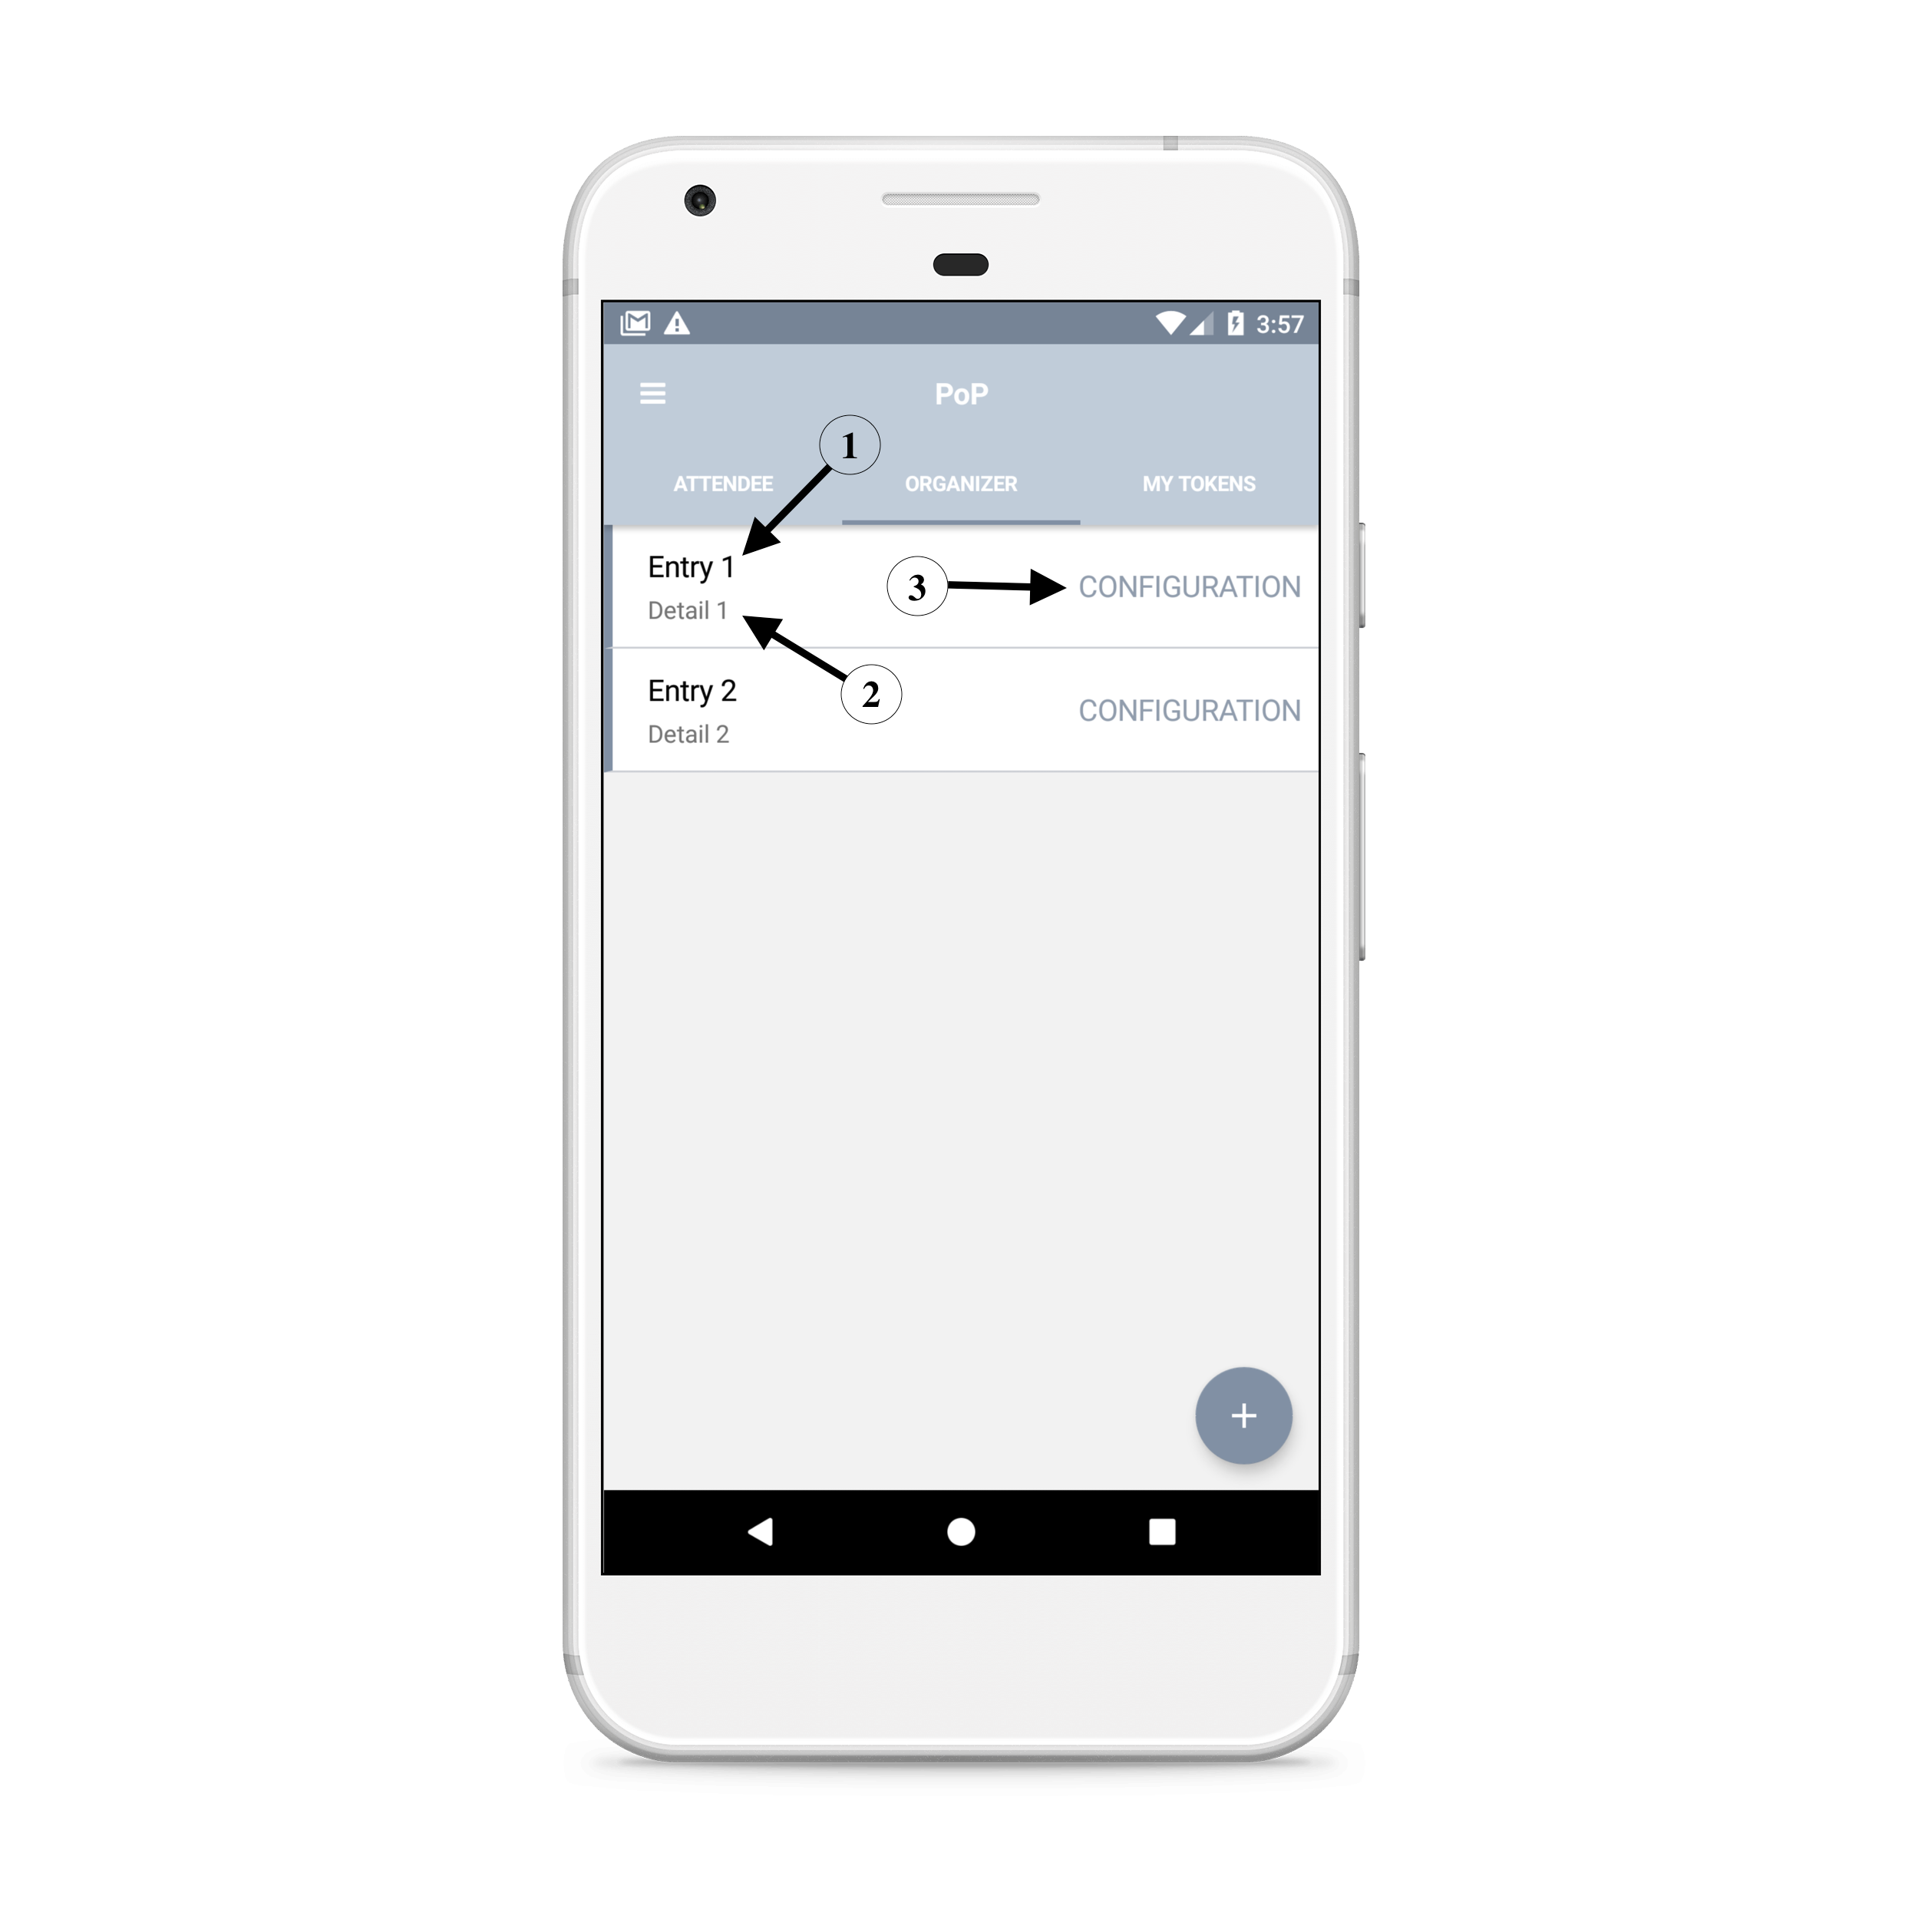
\includegraphics[height=0.8\linewidth]{resources/list_ui.png}
	\caption{Example of a typical list in CP-MAC}
	\label{fig:list_ui}
\end{figure}

\subsection{QR Code Presentation}
The modal page that presents a QR code to other users has also been updated. As this page is frequently used (a lot of information is exchanged by this medium, especially for the Proof-of-Personhood part), a special attention has been ported to create a nice-looking page. The result can be seen on Figure \ref{fig:qrcode_ui} at page \pageref{fig:qrcode_ui}.

\begin{figure}[!ht]
	\centering
	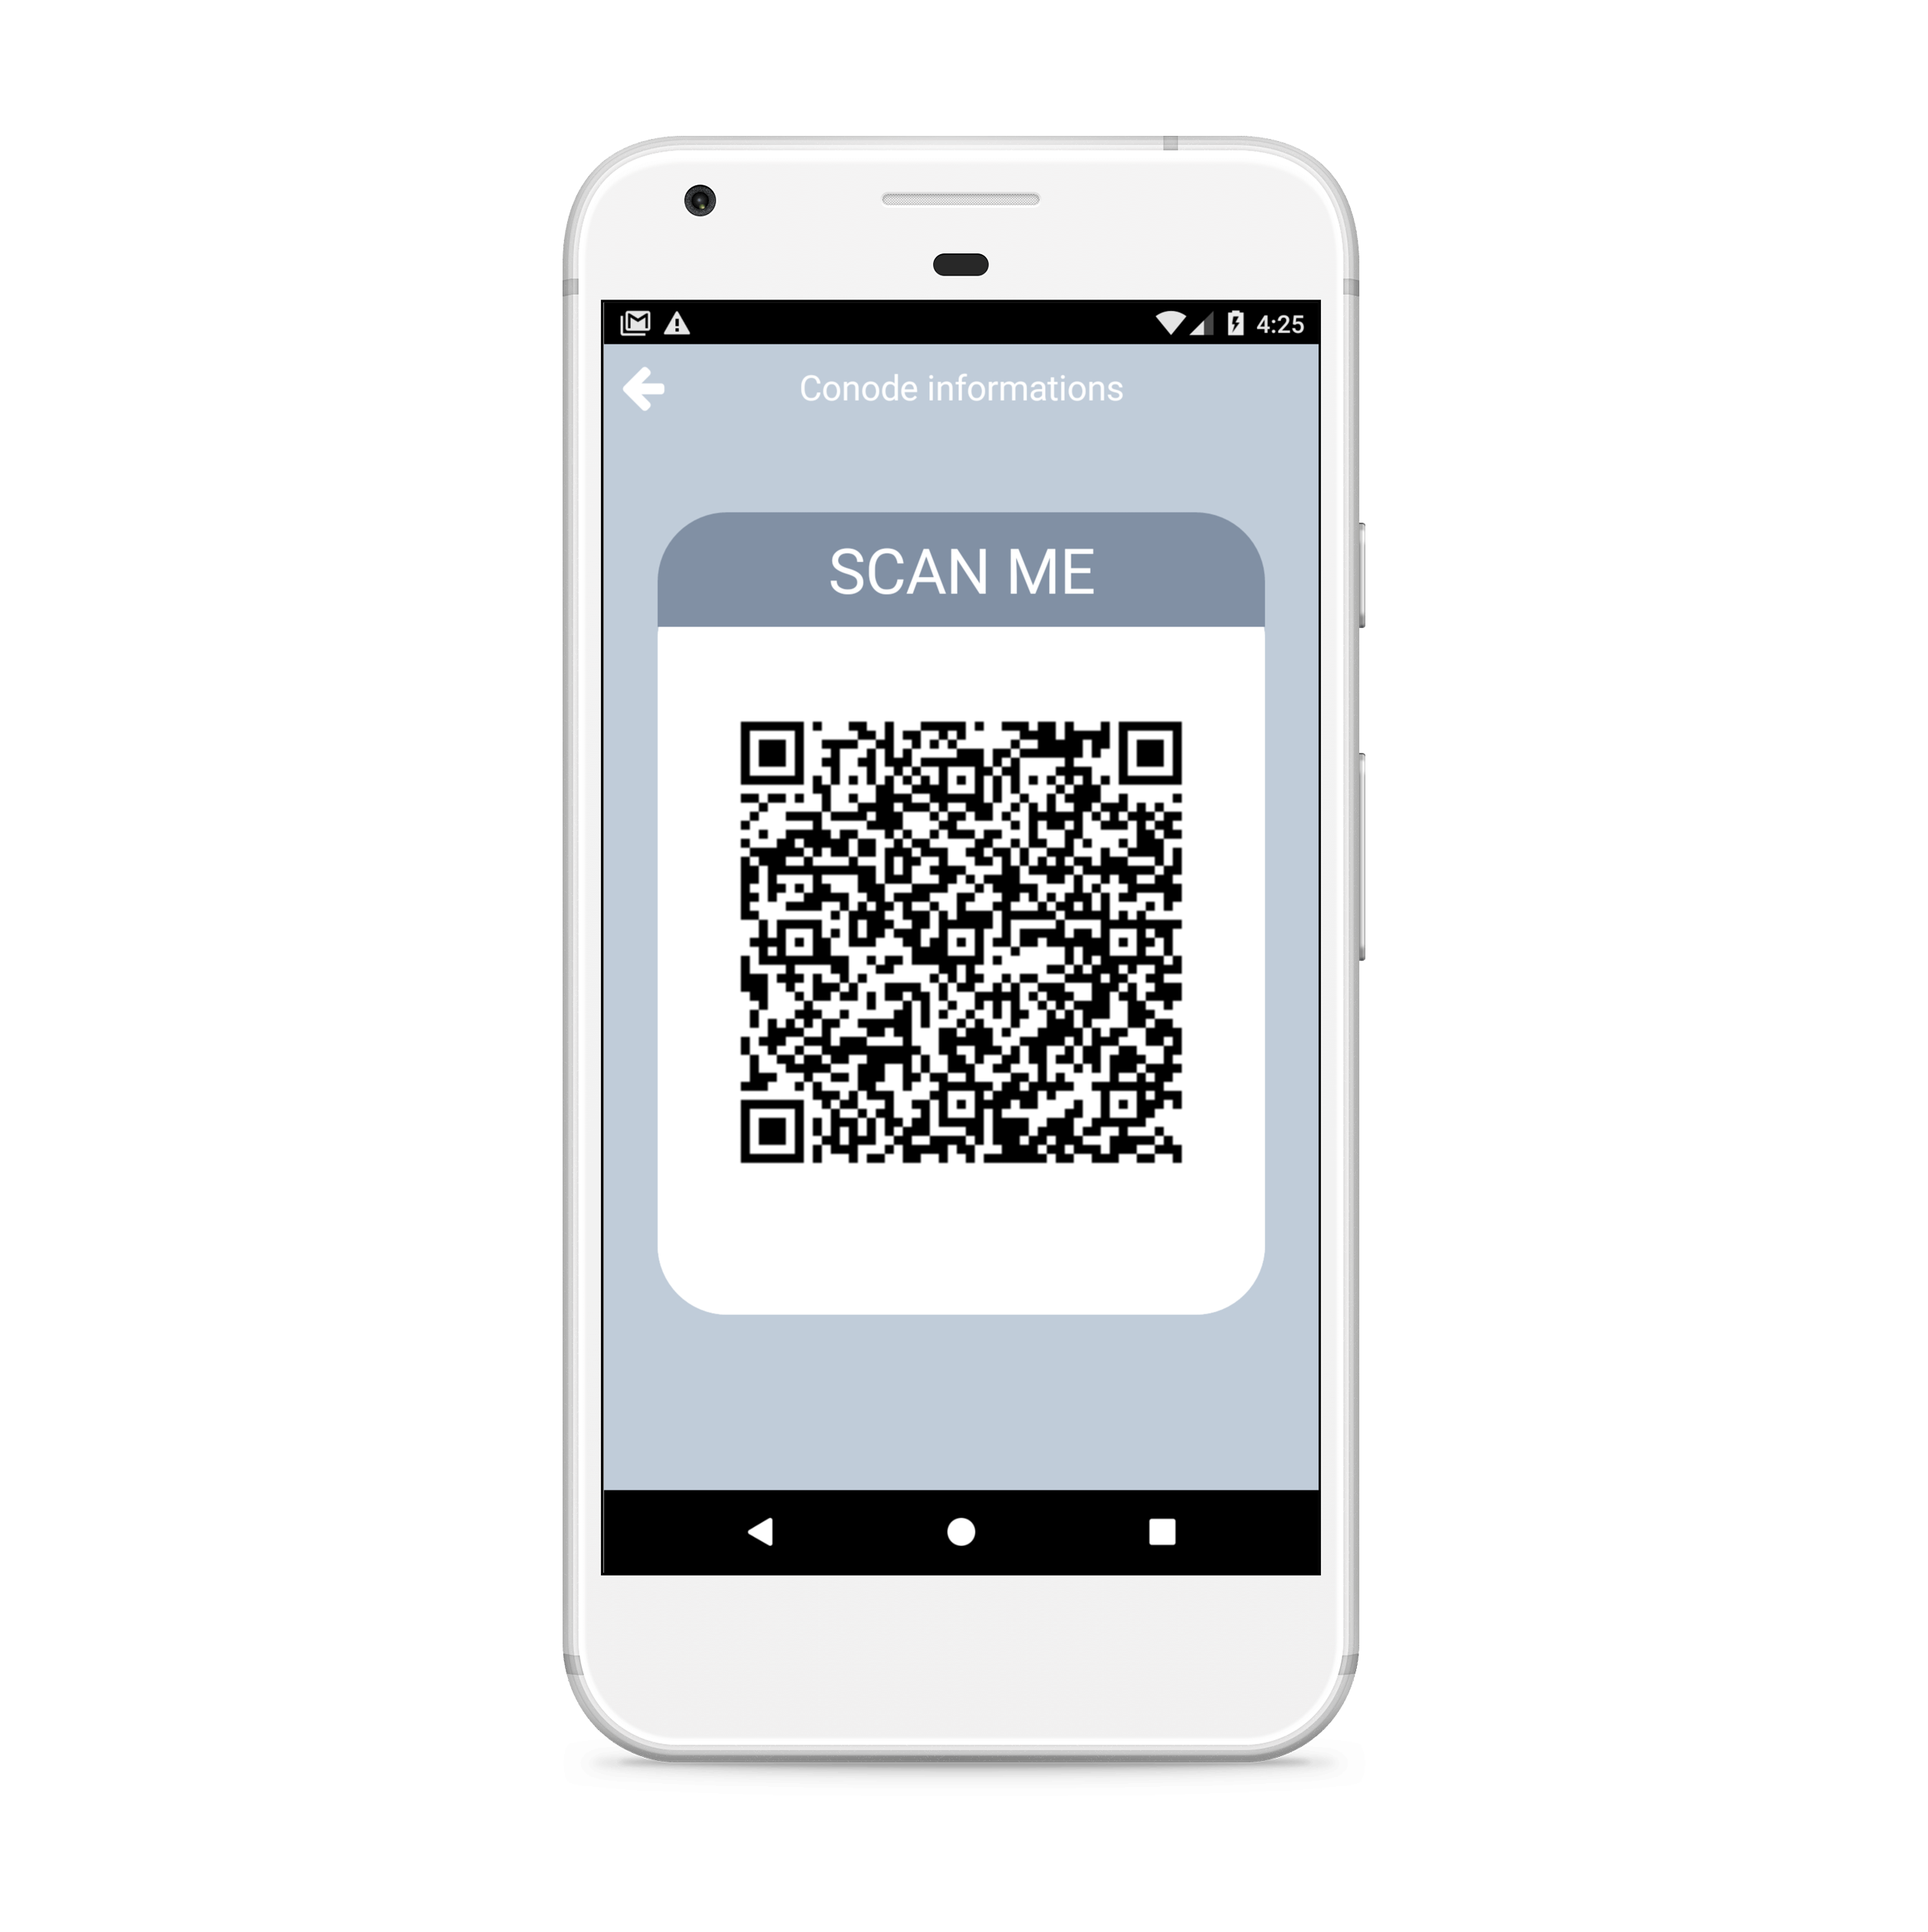
\includegraphics[height=0.8\linewidth]{resources/qrcode_ui.png}
	\caption{Example of the modal QR code presentation page}
	\label{fig:qrcode_ui}
\end{figure}

\section{PoP Part}
\label{sec:pop_part}
The Proof-of-Personhood is the part where most of the work has been focused. Some core features changed, as well as auxiliary functionalities that allows user to spare some useless (repeated) configurations. The major changes will be described in this section. Some minor improvements were also done, such as verifying if the conode was already linked before asking for the PIN.
\subsection{Multiple parties support}
\label{subsec:pop_mult_parties}
As stated previously, CP-MAC formerly handled only one party at the time. This limitation has been removed, and a user can now create, join or delete parties. 
\subsubsection{Implementation}
The singleton object that was taking care of all the party management operations has been converted to a simple object, where each party is now stored in his own directory. On creation, each party gets attributed a unique identifier with UUIDv4\footnote{\url{https://en.wikipedia.org/wiki/Universally_unique_identifier#Version_4_(random)}} format. The directory in which the party is stored is named after this identifier. The general directory structure now looks as follows :

\begin{center}
\begin{minipage}[c]{0.5\textwidth}
\dirtree{%
	.1 pop.
	.2 org.
	.3 RANDOM\_UUID\_1.
	.4 attendees.json.
	.4 conode.json.
	.4 description.json.
	.4 hash.json.
	.3 RANDOM\_UUID\_2.
	.4 ....
}
\end{minipage}
\end{center}

The use of this structure allows CP-MAC to just iterate over the entries of the \url{org} directory to lists the parties, which can be elegantly implemented in NativeScript as it provides interface to execute an action over each entry of a directory using a callback function. 

\subsubsection{Party statuses}
The PoP part of CP-MAC makes use of the status text abstractly described in section \ref{subsec:lists_ui} to show how the party is progressing across time. As these statuses aren't implemented in the Cothority back-end, here is a presentation of the different statuses and how they are deduced from the available data. Most of the statuses are inferred from the response of the \texttt{\textbf{FetchRequest}} message, that fetches the final statement from a conode :

\begin{description}
	\item[\textbf{\texttt{LOADING}}] is set until a response from the conode is received.
	\item[\textbf{\texttt{CONFIGURATION}}] is set when the returned message is a \texttt{"No config found"} error. It informs that the party is only stored locally, thus the conode don't have knowledge of it. 
	\item[\textbf{\texttt{PUBLISHED}}] is set when the returned message contains a final statement, but its list of attendees is empty. It informs that the party is stored on the conode, but not yet finalized.
	\item[\textbf{\texttt{FINALIZING}}] is set when the returned message contains a final statement, but its signature is empty. It informs that the instruction of finalizing has been given, but not on every conode.
	\item[\textbf{\texttt{FINALIZED}}] is set when the returned message contains a final statement, with a non-empty list of attendees and a signature. It informs that the instruction of finalizing has been given on every conodes.
	\item[\textbf{\texttt{ERROR}}] is set in the other cases. It informs that either the network is unavailable or an error occurred, thus the status of this party is unknown.
\end{description}

By using NativeScript primitive for time operations, the final statement can be regularly polled to give informative statuses to the user.

\subsection{Party proposals}
During the creation of a PoP-Party, its description must be shared through all the organizers. Until now, the chosen temporary solution was to use PasteBin, because the usual way of sharing information in CP-MAC (i.e using QR Code) don't have a sufficient capacity to store a party description. However, this had several drawbacks, such as depending on a third party service or giving public access to the party description.

A new procedure has been designed and works entirely on conodes. The general idea is that whenever an organizer publishes a party, the leader conode is used to propagate the description to the other conodes of the party. This way, the rest of the organizers can poll their conode and retrieve the description directly into CP-MAC. The configuration can then be opened in the standard party configuration page of CP-MAC, as seen on Figure \ref{fig:pop_config_ui} at page \pageref{fig:pop_config_ui}.

\begin{figure}[t]
	\centering
	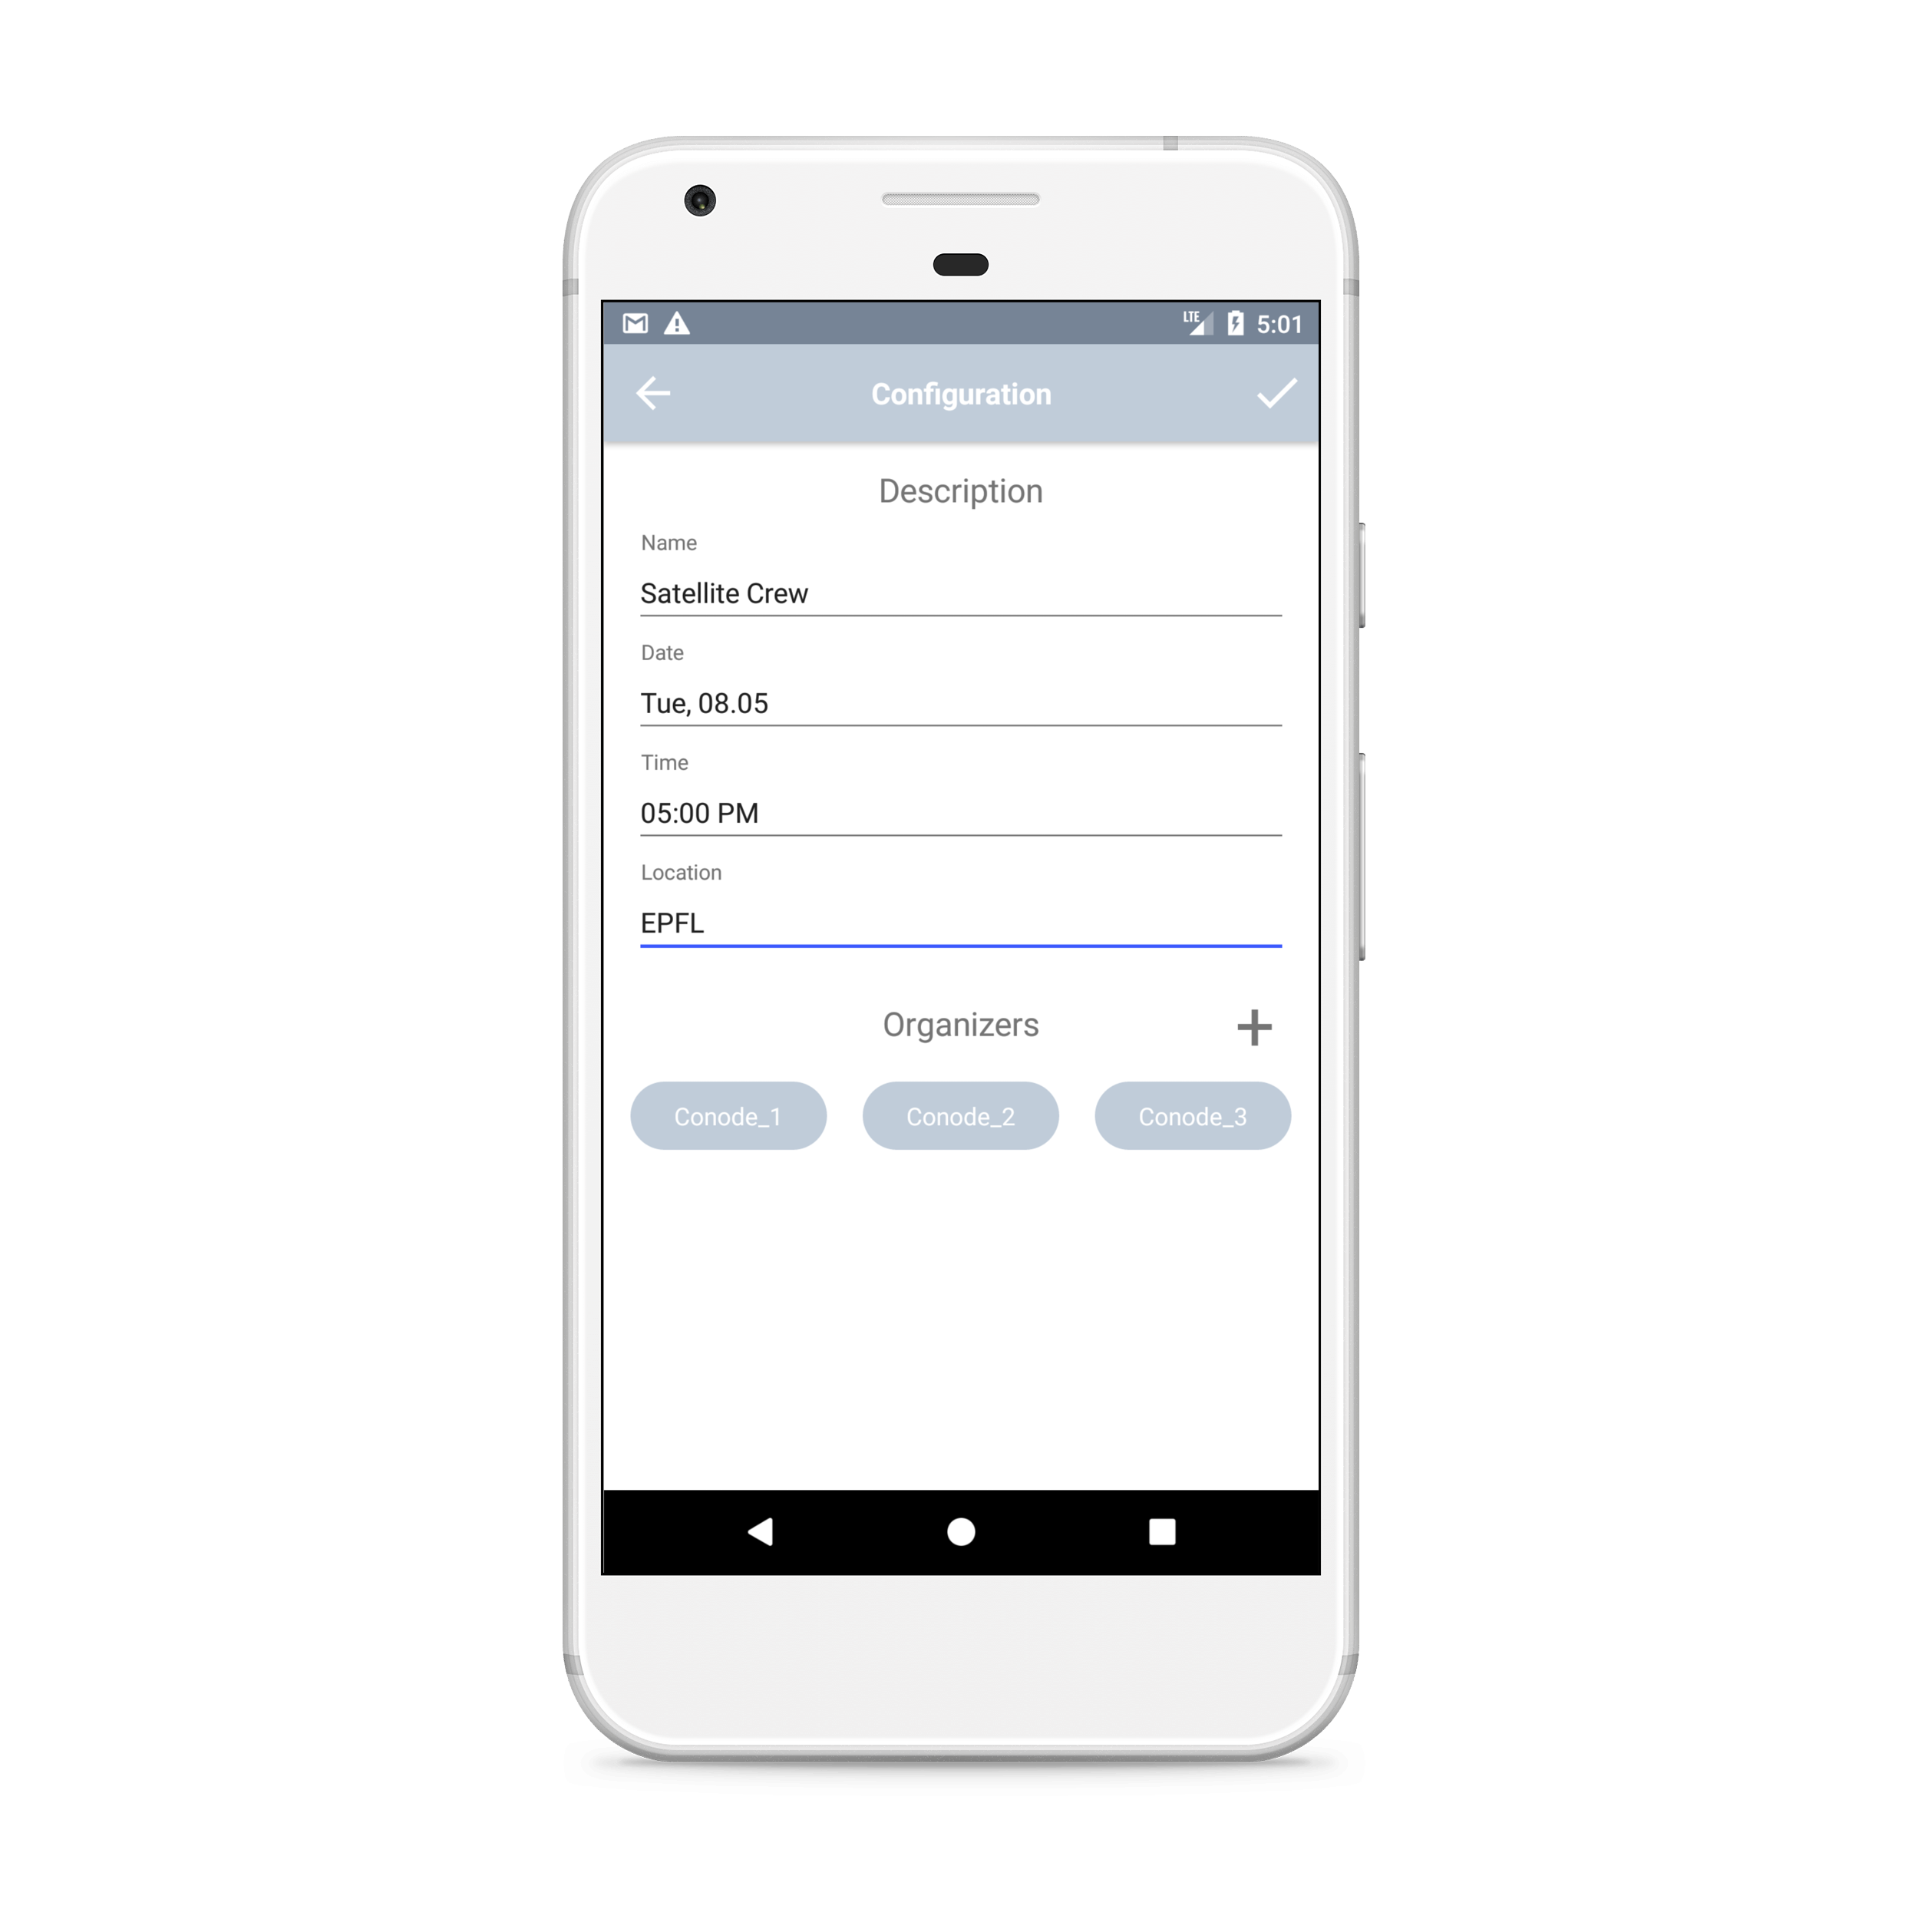
\includegraphics[height=0.8\linewidth]{resources/pop_config_ui.png}
	\caption{Example of a party configuration}
	\label{fig:pop_config_ui}
\end{figure}

\subsubsection{Implementation}
To achieve this, one message behavior has been updated in the Cothority back-end, and a new one has been added :
\begin{description}
	\item[StoreConfig] has been updated : besides storing a configuration on the conode, it will check if the conode is the leader one (i.e if it's the first one in the roster) and if so, it propagates the description to the rest of the roster. The conodes that receive the description will store it until it has been confirmed with \texttt{\textbf{StoreConfig}} within a maximum time period of one hour.
	\item[GetProposals] has been added: it retrieves every party proposals available on the conode.
\end{description}
\begin{figure}
	\centering
	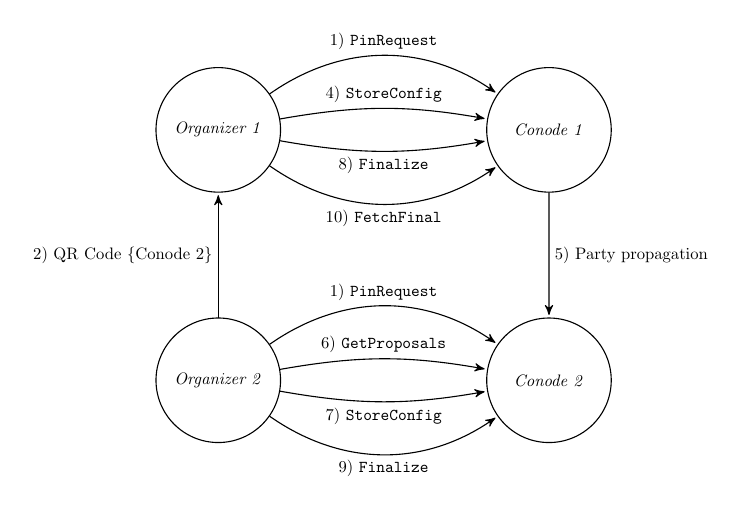
\begin{tikzpicture}[->,>=stealth',shorten >=1pt,node distance=7cm,
scale = 0.6,transform shape, state/.style={circle, draw, minimum size=+75pt}]

\node[state] (Organizer 1) {\textit{Organizer 1}};
\node[state] (Conode 1) [right of=Organizer 1] {\textit{Conode 1}};
\node[state] (Organizer 2) [below of=Organizer 1, yshift=1.7cm] {\textit{Organizer 2}};
\node[state] (Conode 2) [right of=Organizer 2] {\textit{Conode 2}};

\path (Organizer 1) edge [bend left=35]              node [above] {1) \texttt{PinRequest}} (Conode 1)
(Organizer 1) edge [bend left=10]             node [above] {4) \texttt{StoreConfig}} (Conode 1)
(Organizer 1) edge [bend right=10]             node [below] {8) \texttt{Finalize}} (Conode 1)
(Organizer 1) edge [bend right=35]             node [below] {10) \texttt{FetchFinal}} (Conode 1)
(Organizer 2) edge             node [left]{2) QR Code \{Conode 2\}} (Organizer 1)
(Organizer 2) edge [bend left=35]              node [above] {1) \texttt{PinRequest}} (Conode 2)
(Organizer 2) edge [bend left=10]              node [above] {6) \texttt{GetProposals}} (Conode 2)
(Organizer 2) edge  [bend right=10]           node [below] {7) \texttt{StoreConfig}} (Conode 2)
(Organizer 2) edge [bend right=35]             node [below] {9) \texttt{Finalize}} (Conode 2)
(Conode 1) edge              node [right] {5) Party propagation} (Conode 2);

\end{tikzpicture}
	\caption{Graph of a party proposition and retrieval}
	\label{fig:proposal_graph}
\end{figure}
More specifically, here is the typical workflow that might happen for the complete creation of a party involving two organizers (Organizer 1 / Organizer 2) with their respective conode (Conode 1 / Conode 2). The numbers refer to the Figure \ref{fig:proposal_graph} at page \pageref{fig:proposal_graph}, where each link represents either an action or a message to the Cothority back-end.

\begin{enumerate}
	\item Each organizer authenticate to their respective conode
	\item \textit{Organizer 2} presents a QR Code containing his conode information, \{Conode 2\}
	\item \textit{Organizer 1} creates a new party and adds \textit{Organizer 2} to it by scanning the QR Code he is presenting
	\item \textit{Organizer 1} can then publish the party to his conode
	\item \textit{Conode 1} is the leader (first conode in the roster) so it propagates the party description to \textit{Conode 2}
	\item \textit{Organizer 2} can now retrieve the proposals list and notices a new entry
	\item  If the description of the party suits \textit{Organizer 2}, he can publish it to his conode
	\item When the party should end, \textit{Organizer 1} finalizes the party
	\item \textit{Organizer 2} also finalizes the party
	\item Any of the organizers can now fetch the final statement
\end{enumerate}
\subsubsection{Drawbacks and future work}
However, some drawbacks still remain. For example, if an organizer decides to change the description of the party, he has to start over and publish a new party.  This isn't convenient, as this require more time for the organizer than just editing the fields he wants to modify. Also, the other organizers will see a second entry when retrieving the proposals from their conode, which can be confusing and is more error-prone. Additionally, in the current schema, only one organizer decides of the details of the party, and the others only have the choice to accept (publish the party) or refuse (ignore) the current proposition. Again, a better procedure would allow any organizer to propose changes to the party description and when everybody agrees, they could publish it.

A solution to this problem could reside in the Cothorithy Cisc Identity Skipchains. Indeed, Cisc allows users to share key/value data using a private blockchain, on which any member can propose changes and cryptographically vote to accept or refuse changes. A threshold can also be set to define the minimum number of participant who should accept the changes to effectively add them to the blockchain. This would perfectly suit our requirements: each organizer could propose changes that will be reviewed by the rest and when everybody agrees on a description, they can publish it to their conode.
\subsection{Attendee part}
CP-MAC now supports a completely independent section for the management of attendee parties: a user can add a party by scanning the QR Code on the organizer's CP-MAC instance and benefits from the same status monitoring the organizers have. To keep things consistent in the code logic, a new base class \textbf{Party} has been extracted from the common traits of an attendee's party and an organizer's party. Each part can then have their respective \textbf{AttParty} and \textbf{OrgParty}, inherited from the base class.

The implementation of the \textbf{AttParty} will not be described here, as its implementation follows the \textbf{OrgParty} class (multiple parties support, directory structure, status retrieval). The only feature specific to the attendees is the way token are handled.
\subsubsection*{PoP-Token signature}
In contrast to the organizers, attendees make use of the PoP-Tokens, thus, when a party is finalized, the user can choose to generate his PoP-Token. CP-MAC handles the conversion from the final statement to the PoP-Token and makes it available to the user with all the other ones gathered through the previous parties. 

This list of PoP-Tokens will now be useful to the users as it is henceforth possible to sign arbitrary data transmitted using a QR Code and present the resulting signature (with the optional tag) via the same medium. Signatures are generated using (linkable) ring signatures, as described in section \ref{sec:linkable_ring_signature}.

\section{Linkable Ring Signatures}
\label{sec:linkable_ring_signature}
Linkable ring signatures are the missing link in CP-MAC to make the PoP-Tokens useful. As stated before, they're necessary to sign data, but they are also required for the verification.  As this type of digital signatures is not available in KyberJS, it has been necessary to implement it directly in CP-MAC.

\subsection{Implementation}
The sign and verify algorithms are implemented in \textbf{RingSig.js}. It contains also every required auxiliary methods. The execution of the algorithm strictly follows the one implemented in the Kyber Go version and described in \cite{cryptoeprint:2004:027}.  However, as there are major differences between the Go language and JavaScript, some inner mechanisms had to be adapted.

First, as we saw in the BLAKE2 introduction at point \ref{subsubsec:blake2}, BLAKE2Xb is used by Kyber ring signature algorithm but is not available in KyberJS. Two approaches were considered, each one having their drawbacks :

\begin{description}[style=nextline]
	\item[Implement BLAKE2Xb for CP-MAC] As there are several modules in JavaScript that implement BLAKE2b, it is possible to create an instance of BLAKE2Xb without coding the complete algorithm, as a BLAKE2X function can be derived from any BLAKE2 instance (be it BLAKE2b or BLAKE2s). The procedure is described in \cite{aumasson2016blake2x}. This would have assured a complete compliance with the Kyber implementation. However, the remaining time available to complete this project wouldn't have allowed imple\-menting and testing it thoroughly, on top of adding the ring signatures feature.
	\item[Use another hash function] The nearest hash function that I could find is an implementation of BLAKE2Xs implemented in the StableLib\footnote{\url{https://github.com/StableLib/stablelib/tree/master/packages/blake2xs}}. As it provides the same capabilities than BLAKE2Xb, it can be used in ring signature as a replacement. However, the drawback of this solution is that it breaks the compatibility with the Go (reference) version of Kyber. Note that this drawback can be highly moderated by parameterizing the hash function in Kyber and KyberJS, as stated at point \ref{subsec:ring_sig_future_work}. Due to the lack of time, this solution has been chosen. 
\end{description}

The second change that had to be operated concerns the way Kyber marshals its data. This happens during the conversion of the cryptographic elements (points, scalars) to standard byte arrays. Kyber uses a DEDIS library called \textbf{fixbuf}\footnote{\url{https://github.com/dedis/fixbuf}} that allows a fixed length binary encoding of arbitrary Go structures. As there isn't an equivalent library from DEDIS for JavaScript, I implemented a method that reproduces the behavior of \textbf{fixbuf} specifically for ring signature structure. Effectively, here is the Go structure representing an unlinkable ring signature :

\begin{center}
\begin{lstlisting}[language=Golang, caption={Unlinkable ring signature structure}, label={code:ustruct}]
type uSig struct {
	C0 kyber.Scalar 	// generated during the signing process
	S  []kyber.Scalar 	// the length of S equals the number
						// of public keys in the anonymity set
}
\end{lstlisting}
\end{center}
and the one representing a linkable ring signature :
\begin{center}
\begin{lstlisting}[language=Golang, caption={Linkable ring signature structure}, label={code:lstruct}]
type lSig struct {
	C0  kyber.Scalar 	// generated during the signing process
	S  []kyber.Scalar 	// the length of S equals the number
						// of public keys in the anonymity set
	Tag kyber.Point 	// the tag, unique to the signer under 
						// the given scope
}
\end{lstlisting}
\end{center}
According to \textbf{fixbuf}, those elements will be marshaled and concatenated. This can be reproduced in CP-MAC, as KyberJS (like Kyber) allows mar\-shaling cryptographic elements and those structures only contains points or scalar. It's then sufficient to concatenate the resulting byte array of each element, in the right order.

With these changes in mind, the implementation has been done following these steps : first, a specific development version of Kyber for which the hash function is replaced by BLAKE2Xs has been compiled. Also, Kyber and KyberJS have been configured to use a deterministic random function, this way the results between each implementation of the ring signature algorithm can be compared. This facilitated the work as it allowed to verify at each step the coherence of the results.
\subsection{Unit testing}
The tests used to verifiy the \textbf{RingSig.js} implementation are the same as in the Go version, available in the \textbf{sig\_test.go} test suite. Particularly, three scenarios are tested. In each case, signature are tested against the correct and the wrong message, plus the tags are verified (length and validity) when applicable. Here are the different scenarios :
\begin{itemize}
	\item A trivial unlinkable signing process with a single member anonymity set is tested.
	\item An unlinkable signing process with a small anonymity set of three members is also tested. 
	\item  For linkable signatures, an anonymity set of three members is created and a scope is defined. The tags generated when verifying against the good message and a wrong one are then verified.
\end{itemize}
\subsection{Future work}
\label{subsec:ring_sig_future_work}
The most important goal for a future improvement is to make KyberJS fully compatible with Kyber, either by implementing BLAKE2Xb in JavaScript or by parameterizing the hash function. The latter would give a high degree of freedom: for example, it could be possible to create a new suite in Kyber that uses BLAKE2Xs as the hash function. KyberJS would then have to support parameterization of the hash function for a suite, which is currently not the case. However, the former solution have the advantage of being more efficient, as BLAKE2Xb is optimized for 64 bits processor, which begin to be the standard in today smartphones. Of course, by combining the two solutions, we get the best of both world.

\section{BeerCoin Part}
\label{sec:beercoin}
With the different primitives that are now available on CP-MAC, it is possible to create a real use-case. Here, it has been decided to realize a long-running joke at the DEDIS: the creation of a BeerCoin.

\subsection{Description}
The idea behind BeerCoin is that a group of people could each benefit from a free beer every month, week, or day at the expense of someone else. It's also important to preserve the anonymity of the members of the group. For example, it should not be possible to recognize a user from his signature, as well as deducing information about users between two periods. 

Concerning CP-MAC, it should be possible to create a bar from the application, with the possibility to define which group is allowed to get these BeerCoins, and the period before renewal. The bartender could then verify from CP-MAC if a user is allowed to have a beer, and the order history should be kept to allow the BeerCoin supplier to later pay his bill.

\subsection{Implementation}
To implement the BeerCoin, the PoP-Tokens have been used, because, combined with the linkable ring signature, they fulfill all the above require\-ments. Here is the way BeerCoin works in CP-MAC: at first, a user has to create a bar. He can select the group of people which will get the BeerCoins. To simplify this process, CP-MAC will present every group of people from the PoP-Parties in which the user was involved. In fact, when a party gets finalized (let it be an attendee party or an organizer party), the final statement is added to a \textit{bank}\footnote{This \textit{bank} of final statements is in fact the singleton defined in \textbf{PoP.js}, which was already implemented.} of final statements. This way, the user can easily choose for which group he wants to pay the beers. He then chooses a time period and a name for his bar, which concludes the configuration of the bar.

Right after the creation, the directory structure for a bar follows this schema :

\begin{center}
	\begin{minipage}[c]{0.5\textwidth}
		\dirtree{%
			.1 beercoin.
			.2 RANDOM\_UUID\_1.
			.3 bar\_config.json.
			.3 final\_statements.json.
			.3 checked\_clients.json.
			.3 order\_history.json.
			.2 RANDOM\_UUID\_2.
			.3 ....
		}
	\end{minipage}
\end{center}
As we can tell from the \texttt{RANDOM\_UUID} entries, the structure follows the same name generation than a \textbf{Party}\footnote{please refer to point \ref{subsec:pop_mult_parties} for more details.}. Also, here is the usage of each file :
\begin{description}
	\item[bar\_config.json] stores the bar information described above. It also stores the beginning date of the last period. If the difference between the current date and the last reset date is bigger than the defined period for this bar, the list of already seen clients should be reset, and the beginning date updated to reflect the current period.
	\item [final\_statements.json] stores the final statement linked to the party re\-presenting the group of people enjoying the BeerCoins. It will be used to verify the signatures of the clients.
	\item[checked\_clients.json] contains the list of the already seen clients. Their tags are saved in this list (see point \ref{subsubsec:bar_client_verif} for detailed explanations).
	\item[order\_history.json] contains the date of each order that still has to be paid. It can be emptied from the user interface, when all the beers have been paid.
\end{description}

\subsubsection{Client verification}
\label{subsubsec:bar_client_verif}
Once the bar is set up, the verification of a client is pretty straightforward: he first has to scan a QR Code containing the bar information, composed of a nonce and a linkage scope. The linkage scope must be unique for that period, as it will allow the bar to recognize if a client came twice in the same period. Hence, the linkage scope is generated as follows :
\begin{gather}
scope = bar\_name \Vert frequency \Vert year \Vert month \Vert day \\
frequency \in \lbrace daily, weekly, monthly \rbrace \nonumber
\end{gather}
For example, a bar called Satellite that offers a free beer every day for its members would generate the linkage scope \textit{Satellitedaily201868}, assuming the current date is June 8th 2018. The client now signs the nonce with his private key and the linkage scope. The bartender scans a QR Code containing the signature, which is then verified using the final statement public keys as the group of anonymity. If the resulting tag is already in the list of checked clients or if the signature is not valid, the bar refuses the order. Otherwise, the tag is added to the checked clients list, and a new order is logged in the history.

\subsection{Drawbacks and future work}
One of the drawback of this system is the combination of ring signatures with QR Code. Indeed, as we have seen in the listing \ref{code:lstruct} (page \pageref{code:ustruct}), one of the array size in the signature is proportional to the number of public keys in the anonymity set. However, QR Code maximal capacity is $2954$ bytes\footnote{\url{http://www.qrcode.com/en/about/version.html}}, which could be exceeded depending on the number of member in the group.

But is this limit really constraining ? Let's consider a real-world case: CP-MAC bar implementation use the \texttt{edwards25519} curve of KyberJS for the ring signatures. On it, points and scalars are marshaled to 32 bytes long arrays. Again, by referring to listing \ref{code:lstruct}, we can deduce the following inequality :

\begin{align}
	\label{eq:max_qr_pk}
	32 + 32 + 32*n = 32 * n + 64 &\leq 2954 \\
	\implies n &\leq 90.3125
\end{align}
where $n$ is the number of member in the anonymity set. 

From (3) we get that the maximum size of an anonymity set is 90. In CP-MAC, this wouldn't really be an annoying boundary, however, in a real-world situation, this could cause troubles.

A lot of new features could be thought for future work, such as integrating an in-app payment method, or even by allowing people to exchange BeerCoins as any other decentralized token. It could also be possible to work on the drawback explained above, for example by modifying the protocol and integrating a conode as intermediary. CP-MAC would then just serves as a control board, while all the signing processes and signature exchanges are done directly between the client and the conode.

\section{Installation}
Note: This project's code is currently on a branch. It is planned to be merged into the main branch. The instructions below assume the code has been merged. \\\\
A working installation of Go is required to run OmniLedger. The project is in the \texttt{omniledger} directory of Cothority. The Cothority code, which contains the code of this project, is freely available to the public at \texttt{https://github.com/dedis/cothority}. The Go package and its dependencies can be downloaded and installed by using the following commands: \texttt{go get github.com/dedis/cothority}, \texttt{go get github.com/dedis/onet}, \texttt{go get github.com/dedis/kyber}. \\\\

\section{Known bugs}
In this section I will describe the bugs that are either present in the application or have been fixed but are worth to be known. As some problems are related to JavaScript modules or directly to NativeScript, it's possible that the fix may not be necessary anymore in the future. This also allows understanding the necessity of the Makefile: by now, every solved bugs that concerns inherent issues of using NativeScript are fixed using patches, which are applied during the installation with the Makefile. For future bug fixes, this approach is recommended as it keeps the structure of the appli\-cation consistent.

\subsubsection*{Already known bugs}
The list of bugs stated in the report describing the first implementation of CP-MAC are still relevant. More precisely, the WebSocket problem on iOS has still not been fixed yet. The complete list can be found in \cite{petrimaire2018}.

\subsubsection*{KyberJS dependencies}
Sometimes, NPM packages such as KyberJS use built-in Node modules (\texttt{crypto}, in our case) that aren't just JavaScript code but make use of primitives that are specific to the platform on which they run (the browser, or Node). For some of them, an equivalent can be found for NativeScript, such as \texttt{nativescript-crypto} for the previous example. But the faulty modules that imports platform-specific packages still need to update all their \lstinline[language=JavaScript]|require()| statements to point to the correct versions. This can be handled by the module \texttt{nativescript-nodeify}, which installs a NativeScript hook\footnote{Hooks are scripts that are executed at specific moments, such as before the compilation begins.} that will traverse every modules and sub-modules to find incorrect \lstinline[language=JavaScript]|require()| calls to non-compatible packages and replace them with their NativeScript version.

However, in his current version\footnote{0.7.0 as of June 2018.}, \texttt{nativescript-nodeify} excludes every package containing an Organization scope, which prevents KyberJS from being converted, as KyberJS package is \texttt{@dedis/kyber-js}. An issue has been opened on GitHub\footnote{\url{https://github.com/EddyVerbruggen/nativescript-nodeify/issues/33}.} to find out why such a rule is applied, but no answer has been given yet. Thus, a patch applied by the Makefile has been created to remove this condition. Future versions of \texttt{nativescript-nodeify} will maybe fix this issue.

\subsubsection*{iOS version delay}
Unfortunately, due to a bug solved very lately during the project, the iOS version of CP-MAC is not as polished as the Android version. Particularly, some details on the UI still need some work, and some instabilities due to the lack of tests are present. However, some work on this platform is planned and will probably fix these details soon. 

The bug that caused this delay was due to the way \texttt{UglifyJS} mangled\footnote{Mangling is the process of optimizing JavaScrit code size, for example by renaming variables or functions to single letters.} the module CothorityJS. The version of the JavaScriptCore used on iOS was reporting two variables for having the same name, though actual JavaScript specifications on variable scope should allow this case. This was fixed by setting some specifics flags on \texttt{UglifyJS} to prevent this situation\footnote{More details can be read at \url{https://bugs.webkit.org/show_bug.cgi?id=171041}.}.



\clearpage
\printbibliography

\end{document}
